% Standalone architecture diagram for the M.Tech Phase-1 report.
% Compile:  pdflatex system_architecture.tex   ->  system_architecture.pdf
% The resulting tight-bbox vector PDF is included by main.tex (\includegraphics).
% Layout: two VERTICAL pillars (A left, B right); center gap carries the closed
% loop; right side = OpenAI; left side = the two upward returns to Supabase/CAL.
\documentclass[border=12pt]{standalone}
\usepackage[T1]{fontenc}
\usepackage{helvet}
\renewcommand{\familydefault}{\sfdefault}
\usepackage{tikz}
\usetikzlibrary{positioning,fit,backgrounds,arrows.meta,shapes.geometric,calc}

% ---- palette (matches the mermaid styling) -------------------------------
\definecolor{blueStroke}{HTML}{1D4ED8}
\definecolor{blueFill}{HTML}{EFF6FF}
\definecolor{paFill}{HTML}{EAF2FE}
\definecolor{purpStroke}{HTML}{6D28D9}
\definecolor{purpFill}{HTML}{FAF5FF}
\definecolor{greenStroke}{HTML}{047857}
\definecolor{greenFill}{HTML}{ECFDF5}
\definecolor{slate}{HTML}{475569}
\definecolor{slateFill}{HTML}{F1F5F9}
\definecolor{grey}{HTML}{9CA3AF}
\definecolor{greyText}{HTML}{6B7280}
\definecolor{greyFill}{HTML}{F2F2F2}
\definecolor{loopClr}{HTML}{B45309}
\definecolor{inkText}{HTML}{1F2937}

\begin{document}
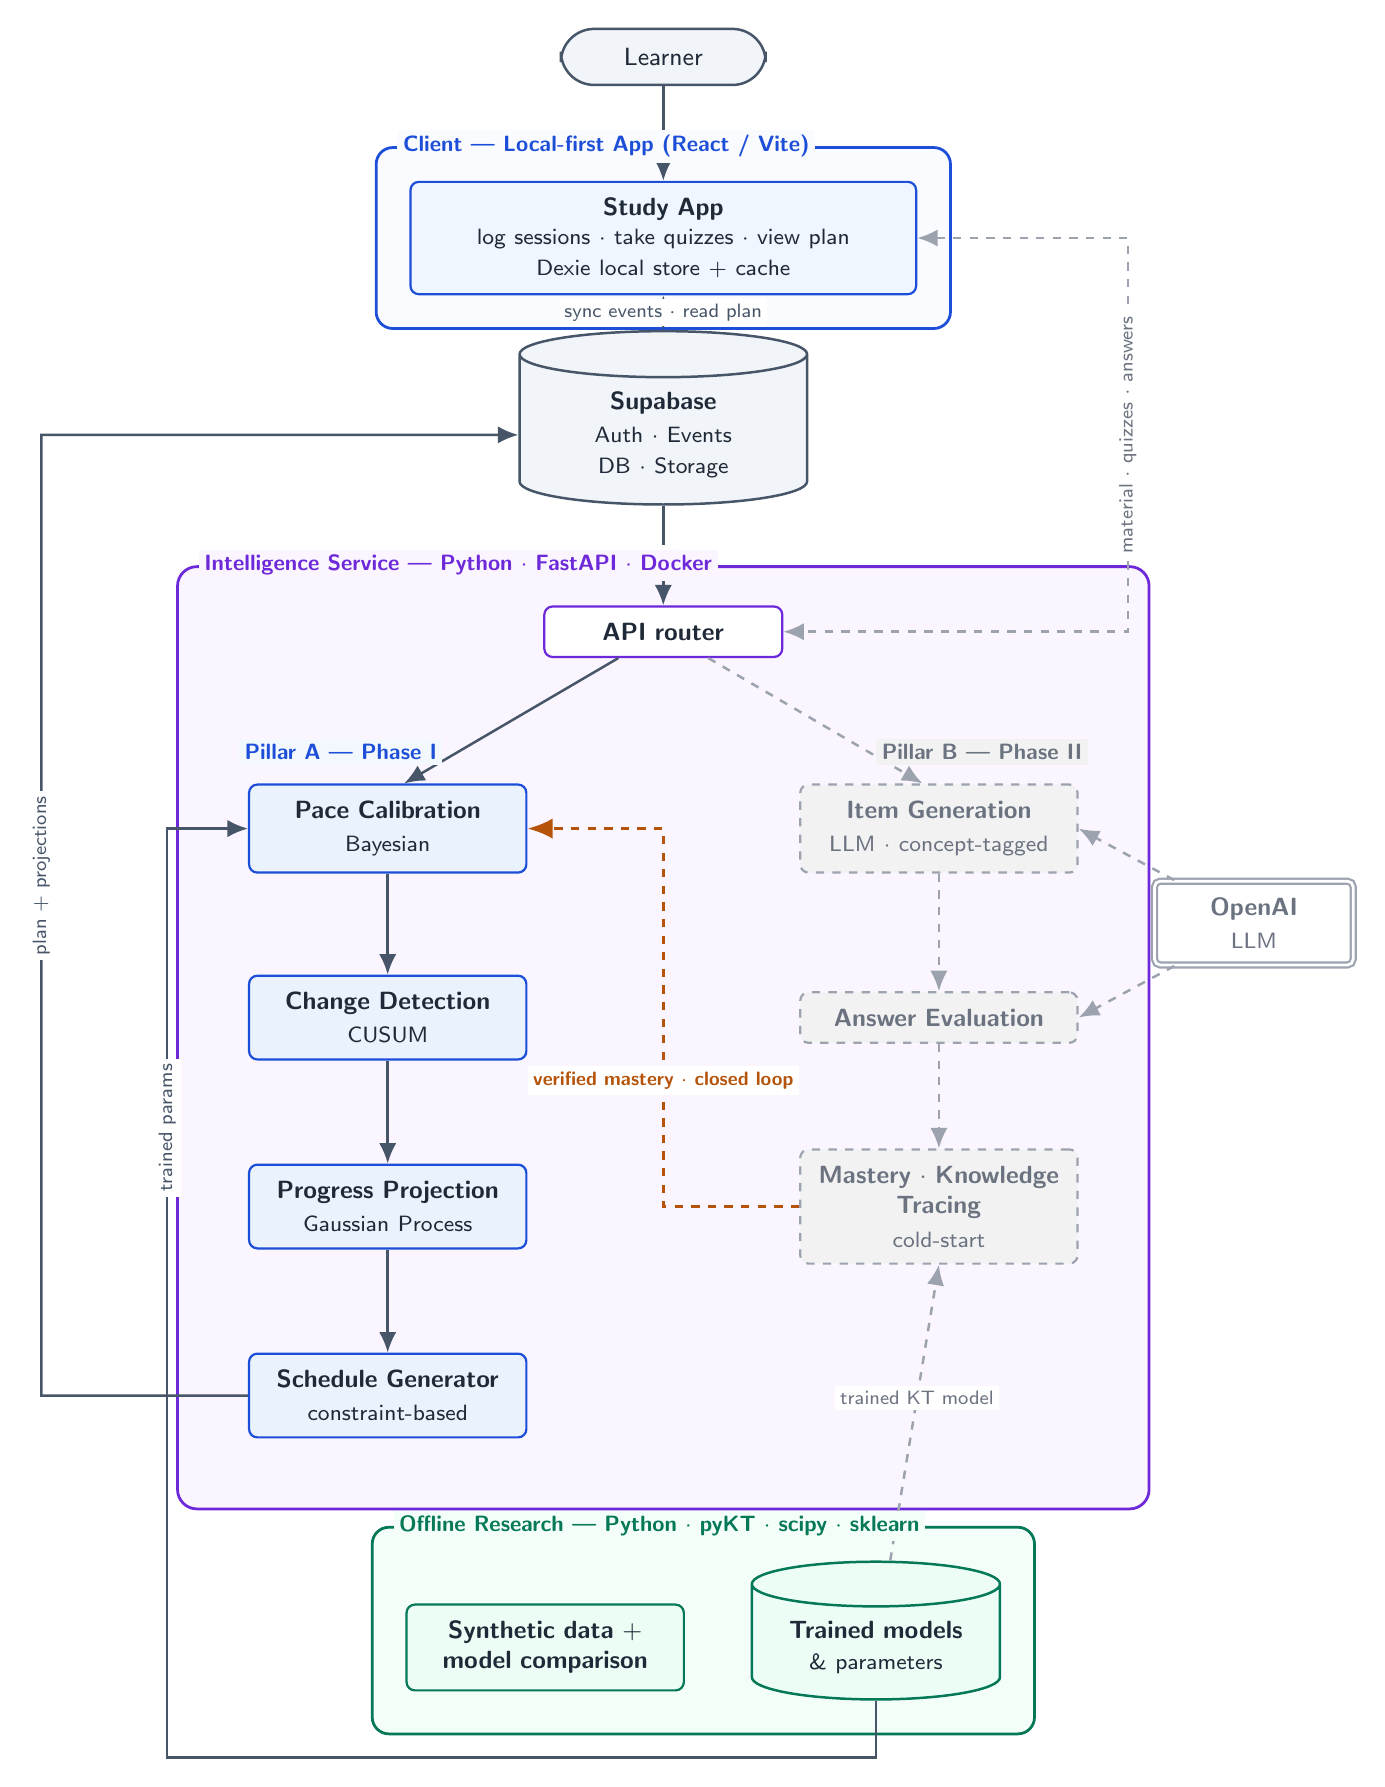
\begin{tikzpicture}[
  font=\small,
  every node/.style={text=inkText},
  box/.style={rounded corners=3pt, draw, line width=0.8pt, align=center,
              inner sep=6pt, text width=3.1cm, fill=white},
  proc/.style={box, draw=blueStroke, fill=paFill},
  phase2/.style={box, draw=grey, dashed, fill=greyFill, text=greyText},
  hub/.style={cylinder, shape border rotate=90, aspect=0.16, draw=slate,
              line width=0.9pt, fill=slateFill, align=center, inner sep=5pt,
              text width=3.3cm, minimum height=1.5cm},
  actor/.style={rounded corners=12pt, draw=slate, line width=0.9pt,
                fill=slateFill, align=center, inner sep=7pt, minimum width=2.6cm},
  ext/.style={draw=grey, line width=0.8pt, double, double distance=1pt,
              rounded corners=2pt, align=center, inner sep=6pt,
              text width=2.1cm, fill=white, text=greyText},
  router/.style={box, draw=purpStroke, fill=white, text width=2.6cm},
  title/.style={font=\footnotesize\bfseries},
  % edges
  flow/.style={-{Latex[length=2.6mm,width=2.2mm]}, line width=0.9pt, draw=slate},
  flowbi/.style={{Latex[length=2.6mm,width=2.2mm]}-{Latex[length=2.6mm,width=2.2mm]},
                 line width=0.9pt, draw=slate},
  dflow/.style={-{Latex[length=2.6mm,width=2.2mm]}, line width=0.9pt, dashed, draw=grey},
  dflowbi/.style={{Latex[length=2.6mm,width=2.2mm]}-{Latex[length=2.6mm,width=2.2mm]},
                  line width=0.9pt, dashed, draw=grey},
  loop/.style={-{Latex[length=3.2mm,width=2.6mm]}, line width=1.2pt, dashed, draw=loopClr},
  lbl/.style={font=\scriptsize, fill=white, inner sep=1.8pt, text=slate},
  dlbl/.style={font=\scriptsize, fill=white, inner sep=1.8pt, text=greyText},
]

% ============================ NODES ======================================
\node[actor] (LEARNER) at (3.5,18.6) {Learner};

\node[box, draw=blueStroke, fill=blueFill, text width=6.0cm] (APP) at (3.5,16.3)
  {\textbf{Study App}\\[1pt]\footnotesize log sessions $\cdot$ take quizzes $\cdot$ view plan\\
   \footnotesize Dexie local store $+$ cache};

\node[hub] (SB) at (3.5,13.8)
  {\textbf{Supabase}\\[1pt]\footnotesize Auth $\cdot$ Events DB $\cdot$ Storage};

\node[router] (ROUTER) at (3.5,11.3) {\textbf{API router}};

% Pillar A (Phase I) -- left column, flows downward
\node[proc] (CAL)  at (0,8.8) {\textbf{Pace Calibration}\\[1pt]\footnotesize Bayesian};
\node[proc] (DET)  at (0,6.4) {\textbf{Change Detection}\\[1pt]\footnotesize CUSUM};
\node[proc] (PROJ) at (0,4.0) {\textbf{Progress Projection}\\[1pt]\footnotesize Gaussian Process};
\node[proc] (SCH)  at (0,1.6) {\textbf{Schedule Generator}\\[1pt]\footnotesize constraint-based};

% Pillar B (Phase II) -- right column, flows downward
\node[phase2] (GEN)  at (7,8.8) {\textbf{Item Generation}\\[1pt]\footnotesize LLM $\cdot$ concept-tagged};
\node[phase2] (EVAL) at (7,6.4) {\textbf{Answer Evaluation}};
\node[phase2] (KT)   at (7,4.0) {\textbf{Mastery $\cdot$ Knowledge}\\\textbf{Tracing}\\[1pt]\footnotesize cold-start};

% Research (offline) -- bottom, feeds both columns upward
\node[box, draw=greenStroke, fill=greenFill] (PIPE) at (2.0,-1.6)
  {\textbf{Synthetic data $+$}\\\textbf{model comparison}};
\node[cylinder, shape border rotate=90, aspect=0.18, draw=greenStroke,
      line width=0.9pt, fill=greenFill, align=center, inner sep=5pt,
      text width=2.8cm, minimum height=1.3cm] (ART) at (6.2,-1.6)
  {\textbf{Trained models}\\\footnotesize \& parameters};

% External
\node[ext] (OAI) at (11.0,7.6) {\textbf{OpenAI}\\[1pt]\footnotesize LLM};

% ====================== CONTAINER BOXES (background) =====================
\begin{scope}[on background layer]
  \node[draw=blueStroke, line width=1pt, rounded corners=6pt, fill=blueFill!40,
        fit=(APP), inner sep=12pt] (clientBox) {};

  \node[draw=blueStroke, line width=0.9pt, rounded corners=6pt, fill=paFill!55,
        fit=(CAL)(DET)(PROJ)(SCH), inner sep=11pt] (paBox) {};

  \node[draw=grey, dashed, line width=0.9pt, rounded corners=6pt, fill=greyFill,
        fit=(GEN)(EVAL)(KT), inner sep=11pt] (pbBox) {};

  \node[draw=purpStroke, line width=1pt, rounded corners=7pt, fill=purpFill,
        fit=(ROUTER)(paBox)(pbBox), inner sep=14pt] (svcBox) {};

  \node[draw=greenStroke, line width=1pt, rounded corners=6pt, fill=greenFill!60,
        fit=(PIPE)(ART), inner sep=12pt] (resBox) {};
\end{scope}

% ============================ EDGES ======================================
% main vertical spine
\draw[flow] (LEARNER) -- (APP);
\draw[flowbi] (APP) -- (SB) node[lbl, midway]{sync events $\cdot$ read plan};
\draw[flow] (SB) -- (ROUTER) node[lbl, midway]{events};

% router into the two pillars (enter on the inner / centre-facing side)
\draw[flow]  (ROUTER) -- (CAL.70);
\draw[dflow] (ROUTER) -- (GEN.110);

% Pillar A pipeline (vertical)
\draw[flow] (CAL)  -- (DET);
\draw[flow] (DET)  -- (PROJ);
\draw[flow] (PROJ) -- (SCH);

% Pillar B pipeline (vertical)
\draw[dflow] (GEN)  -- (EVAL);
\draw[dflow] (EVAL) -- (KT);

% Schedule -> Supabase (far-left return lane)
\draw[flow] (SCH.west) -- (-4.4,1.6) -- (-4.4,13.8) -- (SB.west);
\node[lbl, rotate=90] at (-4.4,8.2) {plan $+$ projections};

% App <-> router (upper-right detour around Supabase)
\draw[dflowbi] (APP.east) -- (9.4,16.3) -- (9.4,11.3) -- (ROUTER.east);
\node[dlbl, rotate=90] at (9.4,13.8) {material $\cdot$ quizzes $\cdot$ answers};

% OpenAI feeds generation + evaluation (short horizontals from the right)
\draw[dflow] (OAI) -- (GEN.east);
\draw[dflow] (OAI) -- (EVAL.east);

% Research artifacts feed the engines (trained params up the left; KT dashed)
\draw[flow]  (ART.south) -- (6.2,-3.0) -- (-2.8,-3.0) -- (-2.8,8.8) -- (CAL.west);
\node[lbl, rotate=90] at (-2.8,5.0) {trained params};
\draw[dflow] (ART) -- (KT.south) node[dlbl, pos=0.55]{trained KT model};

% closed loop: verified mastery -> calibration (up the centre gap)
\draw[loop] (KT.west) -- (3.5,4.0) -- (3.5,8.8) -- (CAL.east);
\node[font=\scriptsize\bfseries, fill=white, inner sep=2pt, text=loopClr]
      at (3.5,5.6) {verified mastery $\cdot$ closed loop};

% ---- container titles (drawn on top so arrows pass behind the text) -------
\node[title, text=blueStroke, fill=blueFill!40, inner sep=2pt, anchor=west]
      at ([xshift=8pt]clientBox.north west) {Client --- Local-first App (React / Vite)};
\node[title, text=purpStroke, fill=purpFill, inner sep=2pt, anchor=west]
      at ([xshift=8pt]svcBox.north west) {Intelligence Service --- Python $\cdot$ FastAPI $\cdot$ Docker};
\node[title, text=blueStroke, fill=paFill!55, inner sep=2pt, anchor=west]
      at ([xshift=8pt]paBox.north west) {Pillar A --- Phase~I};
\node[title, text=greyText, fill=greyFill, inner sep=2pt, anchor=east]
      at ([xshift=-8pt]pbBox.north east) {Pillar B --- Phase~II};
\node[title, text=greenStroke, fill=greenFill!60, inner sep=2pt, anchor=west]
      at ([xshift=8pt]resBox.north west) {Offline Research --- Python $\cdot$ pyKT $\cdot$ scipy $\cdot$ sklearn};

\end{tikzpicture}
\end{document}
